% =============================================================================
%  REPORTE DE PRÁCTICA — Motor DC con PID + InfluxDB + Grafana
%  Materia de Verano: Internet of Things (IoT)
%  Universidad Panamericana · Ingeniería Mecatrónica · 6.° semestre
%
%  INSTRUCCIONES:
%    1. Abre este archivo en overleaf.com
%    2. Completa TODAS las secciones — las que dicen (tarea) van para el viernes
%    3. Inserta capturas de pantalla donde se indica
%    4. Entrega el PDF compilado + sube el .tex a GitHub
% =============================================================================

\documentclass[11pt, letterpaper]{article}

\usepackage[utf8]{inputenc}
\usepackage[T1]{fontenc}
\usepackage{geometry}
\usepackage{xcolor}
\usepackage{fancyhdr}
\usepackage{titlesec}
\usepackage{enumitem}
\usepackage{parskip}
\usepackage{mdframed}
\usepackage{booktabs}
\usepackage{array}
\usepackage{colortbl}
\usepackage{listings}
\usepackage{pgffor}
\usepackage{amssymb}
\usepackage{float}
\usepackage{graphicx}
\usepackage{hyperref}
\usepackage{multicol}
\usepackage{multirow}
\usepackage{tabularx}

\geometry{top=2.2cm, bottom=2.2cm, left=2.5cm, right=2.5cm}

% ── Colores ───────────────────────────────────────────────────────────────────
\definecolor{upBlue}     {HTML}{2E3A59}
\definecolor{roseMain}   {HTML}{C2547A}
\definecolor{roseLight}  {HTML}{FAE8EF}
\definecolor{tealMain}   {HTML}{0F6E56}
\definecolor{tealLight}  {HTML}{E1F5EE}
\definecolor{amberMain}  {HTML}{854F0B}
\definecolor{amberLight} {HTML}{FAEEDA}
\definecolor{purpleMain} {HTML}{534AB7}
\definecolor{purpleLight}{HTML}{EEEDFE}
\definecolor{influxMain} {HTML}{0A85D1}
\definecolor{influxLight}{HTML}{E0F2FF}
\definecolor{grafanaMain}{HTML}{E05F00}
\definecolor{grafanaLight}{HTML}{FFF0E8}
\definecolor{grayLight}  {HTML}{F5F5F5}
\definecolor{grayMid}    {HTML}{BBBBBB}
\definecolor{codeBack}   {HTML}{F0F4F0}
\definecolor{codeComment}{HTML}{5A7A5A}
\definecolor{codeKeyword}{HTML}{6030A0}
\definecolor{codeString} {HTML}{A05000}

% ── Estilo de código ─────────────────────────────────────────────────────────
\lstdefinestyle{cpp}{
  language=C++, backgroundcolor=\color{codeBack},
  basicstyle=\ttfamily\small,
  keywordstyle=\color{codeKeyword}\bfseries,
  commentstyle=\color{codeComment}\itshape,
  stringstyle=\color{codeString},
  numbers=left, numberstyle=\tiny\color{gray}, numbersep=8pt,
  frame=single, framerule=0.5pt, rulecolor=\color{influxMain},
  breaklines=true, tabsize=2, showstringspaces=false,
  literate={á}{{\' a}}1 {é}{{\' e}}1 {í}{{\' i}}1
           {ó}{{\' o}}1 {ú}{{\' u}}1 {ñ}{{\~ n}}1,
}
\lstdefinestyle{flux}{
  backgroundcolor=\color{influxLight},
  basicstyle=\ttfamily\small\color{black},
  frame=single, framerule=0.8pt, rulecolor=\color{influxMain},
  breaklines=true, tabsize=2, numbers=none,
}
\lstset{style=cpp}

% ── Estilos de sección ────────────────────────────────────────────────────────
\titleformat{\section}
  {\large\bfseries\color{upBlue}}{\thesection.}{0.5em}{}
  [\color{roseMain}\titlerule]
\titleformat{\subsection}
  {\normalsize\bfseries\color{upBlue}}{\thesubsection.}{0.5em}{}
\titleformat{\subsubsection}
  {\normalsize\bfseries\color{roseMain}}{\thesubsubsection.}{0.5em}{}

% ── Encabezado ────────────────────────────────────────────────────────────────
\pagestyle{fancy}
\fancyhf{}
\fancyhead[L]{\small\color{upBlue} Reporte --- Motor PID + InfluxDB + Grafana}
\fancyhead[R]{\small\color{upBlue} Universidad Panamericana}
\fancyfoot[C]{\small\color{gray}\thepage}
\renewcommand{\headrulewidth}{0.4pt}
\renewcommand{\headrule}{%
  \hbox to\headwidth{\color{roseMain}\leaders\hrule height\headrulewidth\hfill}}

% ── Cajas ─────────────────────────────────────────────────────────────────────
\newenvironment{instruccion}{%
  \begin{mdframed}[backgroundcolor=tealLight,linecolor=tealMain,linewidth=1pt,
    innerleftmargin=10pt,innerrightmargin=10pt,
    innertopmargin=6pt,innerbottommargin=6pt]
  \small\textbf{\color{tealMain}Instrucci\'on:}\hspace{4pt}
}{\end{mdframed}}

\newenvironment{pendiente}{%
  \begin{mdframed}[backgroundcolor=amberLight,linecolor=amberMain,linewidth=1pt,
    innerleftmargin=10pt,innerrightmargin=10pt,
    innertopmargin=6pt,innerbottommargin=6pt]
  \small\textbf{\color{amberMain}Pendiente (tarea):}\hspace{4pt}
}{\end{mdframed}}

% ── Líneas de respuesta ───────────────────────────────────────────────────────
\newcommand{\linea}[1][5cm]{\underline{\hspace{#1}}}
\newcommand{\respuesta}[1]{%
  \vspace{4pt}%
  \foreach \i in {1,...,#1}{%
    \noindent\textcolor{grayMid}{\rule{\linewidth}{0.3pt}}\\[10pt]%
  }%
}

\hypersetup{colorlinks=true,linkcolor=upBlue,urlcolor=influxMain}

% =============================================================================
\begin{document}
% =============================================================================

% ── Portada ───────────────────────────────────────────────────────────────────
\begin{center}
  {\color{upBlue}\rule{\linewidth}{1.5pt}}\\[0.3cm]
  {\Large\bfseries\color{upBlue} Reporte de Pr\'actica}\\[0.2cm]
  {\large\bfseries\color{roseMain}
    Pr\'actica: Motor DC con PID conectado a InfluxDB y Grafana}\\[0.15cm]
  {\normalsize Materia de Verano: Internet of Things (IoT)
    $\cdot$ Ingenier\'ia Mecatr\'onica
    $\cdot$ 6.\textdegree\ semestre
    $\cdot$ Universidad Panamericana}\\[0.3cm]
  {\color{roseMain}\rule{\linewidth}{0.8pt}}
\end{center}

\vspace{0.3cm}

\begin{tabular}{rl rl}
  \textbf{Alumno 1:}   & Jaime Valencia Rodríguez&
  \textbf{Alumno 2:}   & Marco Alberto Vázquez Preciado\\[0.5em]
  \textbf{Equipo \#:}  & 4&
  \textbf{Fecha:}      & \today        \\[0.6em]
  \textbf{GitHub:}     & https://github.com/0263136-JVR/Practicas-IoT& & \\
\end{tabular}

\vspace{0.5cm}

% ── Tabla de calificación ─────────────────────────────────────────────────────
\begin{mdframed}[backgroundcolor=grayLight,linecolor=grayMid,linewidth=0.5pt,
  innerleftmargin=12pt,innerrightmargin=12pt,
  innertopmargin=6pt,innerbottommargin=6pt]
  \textbf{\color{upBlue}Tabla de calificaci\'on}
  \hfill{\small\color{gray}(uso exclusivo del profesor)}\\[0.4em]
  \begin{tabular}{lcccccccc}
    \toprule
    \textbf{Secci\'on} &
    Obj. & Marco & Mat. & C\'od. & Result. & An\'al. & Concl. &
    \textbf{Total} \\
    \midrule
    \textbf{Puntos} &
    /2 & /4 & /2 & /4 & /6 & /10 & /4 & \textbf{/32} \\
    \bottomrule
  \end{tabular}
\end{mdframed}

\newpage
\tableofcontents
\newpage

% =============================================================================
\section{Objetivo}
% =============================================================================

\begin{instruccion}
  Describe en 2--3 oraciones el objetivo de esta pr\'actica con
  tus propias palabras. Incluye qu\'e se integr\'o, qu\'e se logra
  monitorear y cu\'al es la utilidad pr\'actica en un sistema industrial.
\end{instruccion}

Crear una conexi\'on estable entre una ESP32, con un broker de intermedio (MQTT), para una visualizaci\'on gr\'afica e interacci\'on con el sistema en l\'inea. Esto con el prop\'osito de que el proyecto se pueda convertir en uno de tipo IoT completo donde el usuario tambi\'en tenga control sobre los datos de control.

\vspace{0.4cm}
% =============================================================================
\section{Marco teórico}
% =============================================================================

\begin{instruccion}
  Explica los conceptos clave con tus propias palabras --- no copies
  definiciones. Cada subsección tiene una pregunta gu\'ia para orientarte.
\end{instruccion}

% ── 2.1 ──────────────────────────────────────────────────────────────────────
\subsection{Controlador PID en un sistema IoT}

\textit{Pregunta gu\'ia: ¿Por qu\'e el PID debe correr en el ESP32
(edge) y no en el servidor, aunque el servidor sea m\'as potente?}

Porque un PID depende enteramente de los intervalos entre la lectura de los datos, es decir que depende de la estabilidad provista por el sistema para aplicar la correci\'on a trav\'es del control, lo que conlleva a que el muestro deba ser estricto y constante. Cosa que si todo el procesado se hace fuera de la ESP32 tenga latencia variable y por ende que dificulte la acción correcta del control. Adem\'as, al ser componente de gran relevancia se debe priorizar que su aplicaci\'on sea inmediata, la rapidez en las respuestas es primordial para un correcto funcionamiento y reducción de errores en cualquier sistema controlado.

\vspace{0.4cm}

% ── 2.2 ──────────────────────────────────────────────────────────────────────
\subsection{El papel de MQTT en el pipeline}

\textit{Pregunta gu\'ia: ¿Qu\'e ventaja tiene publicar por MQTT
en lugar de escribir directo a InfluxDB desde el ESP32?}

El uso de un broker como intermediario entre InfluxDB y la ESP32 es mucho más robusto para cualquier aplicaci\'on IoT porque permite a la ESP32 poder publicar sus datos independientemente si existe alg\'un otro servicio recibiendo la informaci\'on, es decir que si existe alg\'un momento de ca\'ida del InfluxDB el broker ser\'a capaz de guardar los mensajes de la planta. Adem\'as de que MQTT es un protocolo m\'as ligero que el http sobre el que trabaja InfluxDB, lo que ahorra energ\'ia y espacio. Y por \'ultimo podemos agregar que usar un broker de intermedio permite poder tener m\'ultiples consumidores del mismo topic.

\vspace{0.4cm}

% ── 2.3 ──────────────────────────────────────────────────────────────────────
\subsection{InfluxDB como base de datos de series de tiempo}

\textit{Pregunta gu\'ia: ¿Qué son los Fields y los Tags en InfluxDB?
¿Cu\'al de los datos del motor es Field y cu\'al ser\'ia Tag?}

\begin{table}[H]
  \centering
  \begin{tabular}{>{\bfseries}p{3cm}
                  >{\centering\arraybackslash}p{2cm}
                  p{8cm}}
    \toprule
    \textbf{Dato} & \textbf{Field / Tag} & \textbf{Justificaci\'on} \\
    \midrule
    rpm     & Field& Es un valor de lectura numérica variable a través del tiempo que corresponde al comportamiento actual del sistema.\\[1.2em]
    setpoint & Field& Es valor numérico. Se encarga de generar el comportamiento deseable del sistema y es sobre el que se compara el dato de rpm para generar la correción.\\[1.2em]
    error    & Field& Es el resultado numérico de la diferencia entre el setpoint y las rpm. Variable en cada etapa de control.\\[1.2em]
    pwm      & Field& Representa la señal de salida controlada del PID que entra al driver del motor. Consiste en un valor de modulación de voltaje para controlar la rpm del motor.\\[1.2em]
    nodo (nombre del ESP32) & Tag& Es un metadato que indentifica el dispositivo físico de origen que representa al sistema.\\[1.2em]
    \bottomrule
  \end{tabular}
  \caption{Clasificaci\'on de los datos del motor en InfluxDB}
\end{table}

% ── 2.4 ──────────────────────────────────────────────────────────────────────
\subsection{Grafana como herramienta de visualización}

\textit{Pregunta gu\'ia: ¿Grafana almacena datos? ¿Qu\'e ocurre
con los datos si Grafana falla por 5 minutos?}

Grafana es un motor de visualizaci\'on, no una base de datos, por lo que realmente ning\'un dato se perder\'ia. Lo que si suceder\'ia es que durante el periodo de fallo no se podr\'a tener una consulta gr\'afica de los datos, pero eso no significa que los otros servicios ligados al env\'io dejen de funcionar, ellos seguir\'an enviado telemetr\'ia y trabajando con la base de datos. Despu\'es, en la reconexi\'on, se tendr\'an disponibles en Grafana los datos durante el periodo de fallo y todo trabajar\'a con normalidad.

\vspace{0.4cm}

% ── 2.5 ──────────────────────────────────────────────────────────────────────
\subsection{Anti-windup en el controlador PID}

\textit{Pregunta gu\'ia: ¿Qu\'e es el windup del integrador y
c\'omo se ve su efecto en la gr\'afica de RPM en Grafana?}

Para empezar, el windup ocurre cuando la salida del controlador alcanza un l\'imite f\'isico en su actuador, un PWM al 100\%, pero el t\'ermino integral sigue acumulando error sin parar. Lo que gr\'aficamente en Grafana podemos verla como overshoots, una constante del PWM en su valor m\'aximo,  y que es respondido por una ca\'ida al extremo opuesto donde las RPM caen por debajo del Setpoint, se tiene una oscilaci\'on masiva de baja frecuencia alrededor del Setpoint.

\newpage

% =============================================================================
\section{Materiales y equipo}
% =============================================================================

\begin{instruccion}
  Enlista todo el hardware y software utilizado.
  Agrega filas si necesitas.
\end{instruccion}

\begin{table}[H]
  \centering
  \begin{tabular}{clcc}
    \toprule
    \textbf{\#} & \textbf{Componente / Software} &
    \textbf{Cantidad} & \textbf{Observaciones} \\
    \midrule
    1  & Arduino Nano ESP32& 1 & \\[0.4em]
    2  & Motor DC con encoder       & 1 & \\[0.4em]
    3  & Driver DRV8833& 1 & \\[0.4em]
    4  & Sensor de efecto Hall      & 1 & \\[0.4em]
    5  & Fuente de alimentaci\'on del motor & 1 & Voltaje: 10 V\\[0.4em]
    6  & Cable USB-A a USB-C& 1 & \\[0.4em]
    7  & Laptop con VS Code + PlatformIO & 1 & SO: Windows\\[0.4em]
    8  & Docker Desktop             & 1 & Versi\'on: 4.83.0\\[0.4em]
    9  & Mosquitto (broker MQTT)    & 1 & En Docker \\[0.4em]
    10 & Telegraf                   & 1 & En Docker \\[0.4em]
    11 & InfluxDB 2.7               & 1 & En Docker \\[0.4em]
    12 & Grafana 10                 & 1 & En Docker \\[0.4em]
    \bottomrule
  \end{tabular}
\end{table}

% =============================================================================
\section{Diagrama de conexiones y arquitectura}
% =============================================================================

\subsection{Conexiones físicas del hardware}

\begin{instruccion}
  Inserta una foto o diagrama de las conexiones del ESP32 con el
  TB6612FNG, el sensor Hall y el motor. Si lo dibujas a mano,
  toma una foto y adjúntala descomentando las líneas de abajo.
\end{instruccion}

% \begin{figure}[H]
%   \centering
%   \includegraphics[width=0.75\textwidth]{conexiones_hardware.jpg}
%   \caption{Conexiones físicas del sistema de control del motor}
% \end{figure}

\begin{table}[H]
  \centering
  \begin{tabular}{>{\ttfamily\bfseries}p{2.8cm}
                  >{\ttfamily\centering\arraybackslash}p{2.8cm}
                  p{7.5cm}}
    \toprule
    \textbf{Pin DRV8833 / Hall}& \textbf{GPIO ESP32} & \textbf{Funci\'on} \\
    \midrule
    AIN1   & GPIO 3& Direcci\'on bit 1 \\[0.6em]
    AIN2   & GPIO 4& Direcci\'on bit 2 \\[0.6em]
    STBY   & 3.3V (fijo) & Habilitar driver \\[0.6em]
    Encoder A& GPIO 6& Pulsos del encoder 
    \\[0.6em]
    Encoder B& GPIO 7& Pulsos del encoder 
    \\[0.6em]
    \bottomrule
  \end{tabular}
  \caption{Tabla de conexiones --- completa los GPIO que usaste}
\end{table}

\subsection{Diagrama de la arquitectura del pipeline}

\begin{instruccion}
  Dibuja el diagrama de bloques del pipeline completo de tu sistema
  (ESP32 $\to$ MQTT $\to$ Telegraf $\to$ InfluxDB $\to$ Grafana)
  indicando qu\'e dato fluye en cada flecha.
  Puedes usar el espacio de abajo o insertar una imagen.
\end{instruccion}

\vspace{5cm}
 \begin{figure}[H]
   \centering
   
\includegraphics[width=0.85\textwidth]{Practica 3/Pipeline.png}
   \caption{Diagrama a bloques que describe el Pipeline del proyecto desde la ESP32 hasta el espacio gráfico en Grafana}
   \label{fig:serial}
 \end{figure}
\vspace{1cm}

\newpage

% =============================================================================
\section{Código fuente}
% =============================================================================

\begin{instruccion}
  Pega el c\'odigo completo de tu \texttt{main.cpp} final.
  Debe ser el c\'odigo real que subiste al ESP32, con tus
  valores de Kp, Ki, Kd y tus GPIOs. No el c\'odigo de ejemplo.
\end{instruccion}

\subsection{platformio.ini}

\begin{lstlisting}[caption={platformio.ini del proyecto}]
No utilizamos platformio.ini ya que hicimos el codigo completo en la plataforma de ArduinoIDE
\end{lstlisting}

\subsection{main.cpp}

\begin{lstlisting}[caption={main.cpp --- PID + MQTT + publicaci\'on a InfluxDB}]
#include <Arduino.h>
#include <WiFi.h>
#include <PubSubClient.h>
#include <ArduinoJson.h>

// ── Configuración WiFi y MQTT ───────────────────────────────────────────────
const char* WIFI_SSID     = "Jaime_S24_FE";
const char* WIFI_PASSWORD = "abcd1234";
const char* MQTT_BROKER = "10.198.97.186";
const int   MQTT_PORT     = 1883;

const char* TOPIC_TELEMETRIA = "iot/motor/telemetria";
const char* TOPIC_SETPOINT   = "iot/motor/setpoint";

WiFiClient wifiClient;
PubSubClient mqttClient(wifiClient);
bool mqttListo = false;

unsigned long ultimoTiempoMQTT = 0;
const unsigned long INTERVALO_MQTT = 500; // Publicar a MQTT cada 500 ms

// ── Pines de Control del Motor (DRV8833 en Paralelo) ────────────────────────
#define MOTOR_PWM_A  6
#define MOTOR_PWM_B  7

// ── Pines del Encoder del JGA25-370 ─────────────────────────────────────────
#define ENCODER_A    9  // Canal A 
#define ENCODER_B    10  // Canal B 

// ── Configuración Física del Motor y Zona Muerta ────────────────────────────
const float PPR = 374.0; 
const int PWM_MINIMO = 60; // Umbral mínimo para vencer la fricción estática

// ── Configuración de Rampas (Suavizado de velocidad) ────────────────────────
const double PASO_ACELERACION    = 5.0; // Suavidad al subir velocidad
const double PASO_DESACELERACION = 5.0; // Suavidad al bajar velocidad

// ── Variables de Control de Estado ──────────────────────────────────────────
volatile bool sentidoHorario = true;  
volatile bool paroEmergencia = false; 
volatile bool motorEncendido = false;  // Guarda el estado del motor (Inicia apagado)

bool modoTestActivo = false;           // Bandera para el Modo Test
unsigned long tiempoImpresoTest = 0;   // Contador de tiempo del test (hasta 5000ms)

double setpointDestinoRPM = 0.0;       // La velocidad final que el usuario desea (Comando S o MQTT)
double setpointActualRPM = 0.0;        // La velocidad transitoria que usa el PID (para las rampas)

// Variables globales para lectura asíncrona de MQTT
double rpmActualGlobal = 0.0;
int pwmGlobal = 0;

// ── Variables del PID ───────────────────────────────────────────────────────
double kp = 1.5;  // 1.5
double ki = 2.1;  // 0.6
double kd = 0.05; // 0.15

double errorAnterior = 0;
double integral = 0;
double derivativaFiltrada = 0; // Para suavizar picos en la derivada

// ── Variables de Tiempo y Encoder ───────────────────────────────────────────
volatile long encoderPulsos = 0;
unsigned long ultimoTiempoPID = 0;
const unsigned long INTERVALO_PID = 50; 

// ── Funciones de Conectividad ───────────────────────────────────────────────

void conectarWiFi() {
  Serial.printf("\n>> [WIFI] Conectando a '%s'", WIFI_SSID);
  WiFi.begin(WIFI_SSID, WIFI_PASSWORD);
  int intentos = 0;
  while (WiFi.status() != WL_CONNECTED && intentos++ < 40) {
    delay(500);
    Serial.print(".");
  }
  if (WiFi.status() == WL_CONNECTED) {
    Serial.printf("\n>> [WIFI] OK - IP: %s\n", WiFi.localIP().toString().c_str());
  } else {
    Serial.println("\n>> [WIFI] FALLO - Continuando offline (Modo Local)");
  }
}

void mqttCallback(char* topic, byte* payload, unsigned int len) {
  String msg = "";
  for (unsigned int i = 0; i < len; i++) msg += (char)payload[i];

  if (String(topic) == TOPIC_SETPOINT) {
    float sp = msg.toFloat();
    if (sp >= 0) {
      setpointDestinoRPM = sp;
      Serial.printf("\n>> [MQTT] Nuevo objetivo recibido: %.2f RPM\n", setpointDestinoRPM);
    }
  }
}

void conectarMQTT() {
  if (WiFi.status() != WL_CONNECTED) return;
  int intentos = 0;
  while (!mqttClient.connected() && intentos++ < 3) {
    Serial.print(">> [MQTT] Conectando al broker...");
    if (mqttClient.connect("ESP32-Motor-Original")) {
      mqttClient.subscribe(TOPIC_SETPOINT);
      mqttListo = true;
      Serial.println(" OK");
    } else {
      Serial.printf(" fallo (rc=%d)\n", mqttClient.state());
      delay(1000);
    }
  }
}

void publicarTelemetria() {
  if (!mqttListo || !mqttClient.connected()) return;

  StaticJsonDocument<200> doc;
  doc["rpm"]      = round(rpmActualGlobal * 10.0f) / 10.0f;
  doc["setpoint"] = setpointActualRPM; 
  doc["error"]    = round(abs(setpointActualRPM - rpmActualGlobal) * 10.0f) / 10.0f;
  doc["pwm"]      = pwmGlobal;
  doc["nodo"]     = "ESP32-Motor-PID";

  char buf[200];
  serializeJson(doc, buf);
  mqttClient.publish(TOPIC_TELEMETRIA, buf);
}

// ── Interrupciones ──────────────────────────────────────────────────────────

void IRAM_ATTR analizarEncoder() {
  int estadoB = digitalRead(ENCODER_B);
  if (estadoB == HIGH) { encoderPulsos++; } else { encoderPulsos--; }
}

// ── Setup ───────────────────────────────────────────────────────────────────

void setup() {
  Serial.begin(115200);
  while (!Serial) { delay(10); } 

  pinMode(MOTOR_PWM_A, OUTPUT);
  pinMode(MOTOR_PWM_B, OUTPUT);
  
  frenarMotor(); // Seguridad inicial

  pinMode(ENCODER_A, INPUT_PULLUP);
  pinMode(ENCODER_B, INPUT_PULLUP);
  attachInterrupt(digitalPinToInterrupt(ENCODER_A), analizarEncoder, RISING);

  // Inicialización de Red
  conectarWiFi();
  if (WiFi.status() == WL_CONNECTED) {
    mqttClient.setServer(MQTT_BROKER, MQTT_PORT);
    mqttClient.setCallback(mqttCallback);
    mqttClient.setBufferSize(512);
    conectarMQTT();
  }

  // ── Filtro de Arranque ──
  delay(200);                 // Espera a que la tensión de la fuente se estabilice
  encoderPulsos = 0;          // Limpia cualquier pulso falso del interruptor de encendido
  ultimoTiempoPID = millis(); // Sincroniza el reloj del PID
  ultimoTiempoMQTT = millis();

  Serial.println("\n--- ¡Sistema PID IoT con Modo Test Listo! ---");
  imprimirInstrucciones();
}

// ── Loop ────────────────────────────────────────────────────────────────────

void loop() {
  if (mqttListo) mqttClient.loop();
  procesarConsola();

  unsigned long tiempoActual = millis();

  if (tiempoActual - ultimoTiempoPID >= INTERVALO_PID) {
    double dt = (tiempoActual - ultimoTiempoPID) / 1000.0; 
    ultimoTiempoPID = tiempoActual;

    noInterrupts();
    long pulsosAcumulados = encoderPulsos;
    encoderPulsos = 0; 
    interrupts();

    double rps = abs((double)pulsosAcumulados) / (PPR * dt);
    double rpmActual = rps * 60.0;
    rpmActualGlobal = rpmActual;

    bool requierePID = true;

    // ── GESTIÓN DE ESTADOS Y RAMPAS ──
    if (modoTestActivo) {
      if (setpointActualRPM < setpointDestinoRPM) {
        setpointActualRPM += PASO_ACELERACION;
        if (setpointActualRPM > setpointDestinoRPM) setpointActualRPM = setpointDestinoRPM;
      }
    }
    else if (paroEmergencia) {
      frenarMotor();
      setpointActualRPM = 0.0; 
      integral = 0;
      errorAnterior = 0;
      requierePID = false;
      pwmGlobal = 0;
      Serial.print("Target:0.00,Actual:"); Serial.print(rpmActual); Serial.println(",PWM:EMERGENCIA_ESTOP");
    } 
    else if (!motorEncendido) {
      if (setpointActualRPM > 0.0) {
        setpointActualRPM -= PASO_DESACELERACION;
        if (setpointActualRPM < 0.0) setpointActualRPM = 0.0;
      }
      
      if (setpointActualRPM == 0.0) {
        analogWrite(MOTOR_PWM_A, 0);
        analogWrite(MOTOR_PWM_B, 0);
        integral = 0;
        errorAnterior = 0;
        requierePID = false;
        pwmGlobal = 0;
        Serial.print("Target:0.00,Actual:"); Serial.print(rpmActual); Serial.println(",PWM:0_APAGADO");
      }
    } 
    else {
      if (setpointActualRPM < setpointDestinoRPM) {
        setpointActualRPM += PASO_ACELERACION;
        if (setpointActualRPM > setpointDestinoRPM) setpointActualRPM = setpointDestinoRPM;
      } 
      else if (setpointActualRPM > setpointDestinoRPM) {
        setpointActualRPM -= PASO_DESACELERACION;
        if (setpointActualRPM < setpointDestinoRPM) setpointActualRPM = setpointDestinoRPM;
      }
      
      if (setpointActualRPM == 0.0 && setpointDestinoRPM == 0.0) {
        analogWrite(MOTOR_PWM_A, 0);
        analogWrite(MOTOR_PWM_B, 0);
        integral = 0;
        errorAnterior = 0;
        requierePID = false;
        pwmGlobal = 0;
        Serial.print("Target:0.00,Actual:"); Serial.print(rpmActual); Serial.println(",PWM:0_REPOSO");
      }
    }

    // ── EJECUCIÓN DEL CONTROLADOR PID ──
    if (requierePID) {
      double error = setpointActualRPM - rpmActual;
      
      // 1. Banda Muerta (Deadband): Previene que el motor "vibre" cazando errores microscópicos
      const double BANDA_MUERTA = 1.0; // Si el error es menor a 1 RPM, lo damos por bueno
      if (abs(error) < BANDA_MUERTA) {
          error = 0; 
      }

      // 2. Cálculo Proporcional y Derivativo (con Filtro Paso Bajo)
      double P = kp * error;
      
      double derivativaCruda = (error - errorAnterior) / dt;
      // Filtro paso bajo para la derivada (alfa = 0.3)
      derivativaFiltrada = 0.3 * derivativaCruda + 0.7 * derivativaFiltrada;
      double D = kd * derivativaFiltrada;
      
      errorAnterior = error;

      // 3. Integración Condicional (Anti-Windup Avanzado)
      // Calculamos cuánto control aplicaríamos en este ciclo
      double controlTeorico = P + D + (ki * (integral + error * dt));
      
      // Límites efectivos de control (descontando el mínimo para vencer la inercia)
      double limiteSup = 255.0 - PWM_MINIMO;
      double limiteInf = 0.0;
      
      // Solo sumamos a la integral si NO estamos saturados, o si el error tiende a reducir la saturación
      bool saturadoArriba = (controlTeorico >= limiteSup && error > 0);
      bool saturadoAbajo  = (controlTeorico <= limiteInf && error < 0);
      
      if (!saturadoArriba && !saturadoAbajo) {
          integral += error * dt;
      }

      // Mantenemos tu límite estático de seguridad
      if (ki != 0) { integral = constrain(integral, -255.0 / ki, 255.0 / ki); }
      
      // 4. Cálculo final del esfuerzo de control
      double controlU = P + (ki * integral) + D;
      
      int pwmControlado = 0;
      if (controlU > 0) {
        pwmControlado = (int)controlU + PWM_MINIMO;
      } else {
        pwmControlado = PWM_MINIMO; 
      }
      pwmControlado = constrain(pwmControlado, PWM_MINIMO, 255);
      
      pwmGlobal = pwmControlado;
      aplicarMovimiento(pwmControlado);

      // Impresión en formato estándar
      Serial.print("Target:"); Serial.print(setpointActualRPM); Serial.print(",");
      Serial.print("Actual:"); Serial.print(rpmActual); Serial.print(",");
      Serial.print("Error:"); Serial.print(abs(setpointActualRPM - rpmActual)); Serial.print(",");
      Serial.print("PWM:"); Serial.println(pwmControlado);

      // Lógica de finalización del Modo Test
      if (modoTestActivo) {
        tiempoImpresoTest += INTERVALO_PID;
        if (tiempoImpresoTest >= 5000) {
          analogWrite(MOTOR_PWM_A, 0);
          analogWrite(MOTOR_PWM_B, 0);
          
          Serial.println("--- FIN MODO TEST (Motor Apagado) ---");
          Serial.println(">> Esperando 5 segundos de pausa final...");
          Serial.flush();
          
          delay(5000);
          
          modoTestActivo = false;
          motorEncendido = false;
          setpointActualRPM = 0.0;
          integral = 0;
          errorAnterior = 0;
          
          Serial.println(">> Sistema listo para nuevas instrucciones.\n");
        }
      }
    }
  }

  // 3. Bucle de transmisión MQTT
  if (tiempoActual - ultimoTiempoMQTT >= INTERVALO_MQTT) {
    ultimoTiempoMQTT = tiempoActual;
    publicarTelemetria();
    if (mqttListo && !mqttClient.connected()) conectarMQTT();
  }
}

// ── Funciones de Control del Driver DRV8833 ─────────────────────────────────

void aplicarMovimiento(int pwm) {
  if (sentidoHorario) {
    analogWrite(MOTOR_PWM_A, pwm);
    analogWrite(MOTOR_PWM_B, 0);
  } else {
    analogWrite(MOTOR_PWM_A, 0);
    analogWrite(MOTOR_PWM_B, pwm);
  }
}

void frenarMotor() {
  analogWrite(MOTOR_PWM_A, 255);
  analogWrite(MOTOR_PWM_B, 255);
}

// ── Utilidades de Consola Interactiva ───────────────────────────────────────

void imprimirInstrucciones() {
  Serial.println("\n--- COMANDOS DE CONTROL DISPONIBLES ---");
  Serial.println("  S<valor>  : Definir RPM objetivo (Ej: S120)");
  Serial.println("  KP<valor> : Modificar Kp (Ej: KP2.5)");
  Serial.println("  KI<valor> : Modificar Ki (Ej: KI1.8)");
  Serial.println("  KD<valor> : Modificar Kd (Ej: KD0.05)");
  Serial.println("  C         : Ver constantes PID actuales");
  Serial.println("  T         : EJECUTAR MODO TEST (5s con impresiones normalizadas)");
  Serial.println("  R         : ENCENDER / REANUDAR (Modo continuo)");
  Serial.println("  A         : APAGADO GRADUAL (Bajada suave y progresiva)");
  Serial.println("  E         : PARO DE EMERGENCIA (Freno total instantáneo)");
  Serial.println("  D         : Cambiar sentido de giro");
  Serial.println("---------------------------------------\n");
}

void procesarConsola() {
  if (Serial.available() > 0) {
    char comando = Serial.read();
    
    switch (comando) {
      case 'S': case 's': {
        float nuevaVelocidad = Serial.parseFloat();
        if (nuevaVelocidad >= 0) {
          setpointDestinoRPM = nuevaVelocidad;
          Serial.print(">> Objetivo guardado: ");
          Serial.print(setpointDestinoRPM);
          Serial.println(" RPM. Usa 'T' para test de 5s o 'R' para modo continuo.");
        }
        break;
      }
      case 'K': case 'k': {
        delay(5); 
        char subComando = Serial.read();
        float nuevoValor = Serial.parseFloat();
        
        if (nuevoValor >= 0) {
          if (subComando == 'P' || subComando == 'p') {
            kp = nuevoValor;
            Serial.print(">> [PID] Kp actualizado a: "); Serial.println(kp, 4);
          } else if (subComando == 'I' || subComando == 'i') {
            ki = nuevoValor;
            integral = 0; 
            Serial.print(">> [PID] Ki actualizado a: "); Serial.println(ki, 4);
          } else if (subComando == 'D' || subComando == 'd') {
            kd = nuevoValor;
            Serial.print(">> [PID] Kd actualizado a: "); Serial.println(kd, 4);
          }
        }
        break;
      }
      case 'C': case 'c': {
        Serial.println("\n--- VALORES ACTUALES DEL PID ---");
        Serial.print("  Kp = "); Serial.println(kp, 4);
        Serial.print("  Ki = "); Serial.println(ki, 4);
        Serial.print("  Kd = "); Serial.println(kd, 4);
        Serial.println("--------------------------------\n");
        break;
      }
      case 'T': case 't': {
        if (setpointDestinoRPM <= 0) {
          Serial.println(">> [AVISO] Define primero una velocidad objetivo con S<valor> (Ej: S100)");
        } else {
          Serial.println("\n>> [INICIO] Preparando Modo Test...");
          Serial.println(">> Silenciando e iniciando test en 5 segundos...");
          
          for (int i = 5; i > 0; i--) {
            Serial.print(">> "); Serial.print(i); Serial.println("...");
            delay(1000);
          }

          paroEmergencia = false;
          motorEncendido = true;
          modoTestActivo = true;
          
          setpointActualRPM = 0.0;
          integral = 0;
          errorAnterior = 0;
          tiempoImpresoTest = 0;
          
          noInterrupts();
          encoderPulsos = 0;
          interrupts();
          
          ultimoTiempoPID = millis();
          
          Serial.println("\n--- INICIO MODO TEST (5 Segundos) ---");
        }
        break;
      }
      case 'R': case 'r': {
        paroEmergencia = false;
        modoTestActivo = false;
        motorEncendido = true; 
        Serial.println(">> [ESTADO] Sistema ENCENDIDO en modo continuo...");
        break;
      }
      case 'A': case 'a': {
        modoTestActivo = false;
        motorEncendido = false; 
        Serial.println(">> [ESTADO] Iniciando desaceleración controlada...");
        break;
      }
      case 'E': case 'e': {
        paroEmergencia = true;   
        modoTestActivo = false;
        motorEncendido = false;  
        Serial.println(">> [ALERTA] ¡PARO DE EMERGENCIA ACTIVADO! Freno en seco aplicado.");
        break;
      }
      case 'D': case 'd': {
        sentidoHorario = !sentidoHorario;
        integral = 0; 
        Serial.print(">> Sentido cambiado a: ");
        Serial.println(sentidoHorario ? "HORARIO" : "ANTIHORARIO");
        break;
      }
    }
  }
}
\end{lstlisting}

\subsection{Parámetros del PID}

\begin{table}[H]
  \centering
  \begin{tabular}{>{\bfseries}p{3cm}
                  >{\centering\arraybackslash}p{2.5cm}
                  p{7.5cm}}
    \toprule
    \textbf{Par\'ametro} & \textbf{Valor usado} & \textbf{C\'omo lo obtuviste} \\
    \midrule
    $K_p$ & 1.5& Prueba y error\\[1em]
    $K_i$ & 2.1& Prueba y error\\[1em]
    $K_d$ & 0.05& Prueba y error\\[1em]
    Intervalo PID (ms) & 50& Tiempo de ejecucion normal de un PID\\[1em]
    Intervalo MQTT (ms)& 500& Valor bueno para no saturar el MQTT de datos\\[1em]
    PPR (pulsos/vuelta) & 374& Pulsos del motor x Relacion de giro (11 * 34)\\[1em]
    \bottomrule
  \end{tabular}
  \caption{Par\'ametros del sistema de control}
\end{table}

\newpage

% =============================================================================
\section{Resultados}
% =============================================================================

\subsection{Capturas de pantalla del sistema funcionando}

\begin{instruccion}
  Inserta capturas de pantalla de cada uno de los siguientes elementos.
  Para cada una, escribe una oraci\'on describiendo qu\'e muestra.
\end{instruccion}

\subsubsection{Serial Monitor del ESP32}

 \begin{figure}[H]
   \centering
   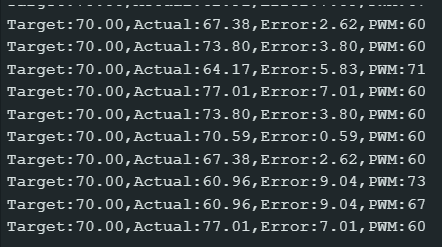
\includegraphics[width=0.85\textwidth]{CapturaSerial.png}
   \caption{Salida del Serial Monitor durante la práctica}
   \label{fig:serial}
 \end{figure}

\textbf{Descripci\'on:}
La captura de pantalla muestra como envia al monitor serial los datos nuestro sistema. De esta forma somos capaces de ver la informacion en el monitor serial.

\subsubsection{Data Explorer de InfluxDB con los datos del motor}

 \begin{figure}[H]
   \centering
   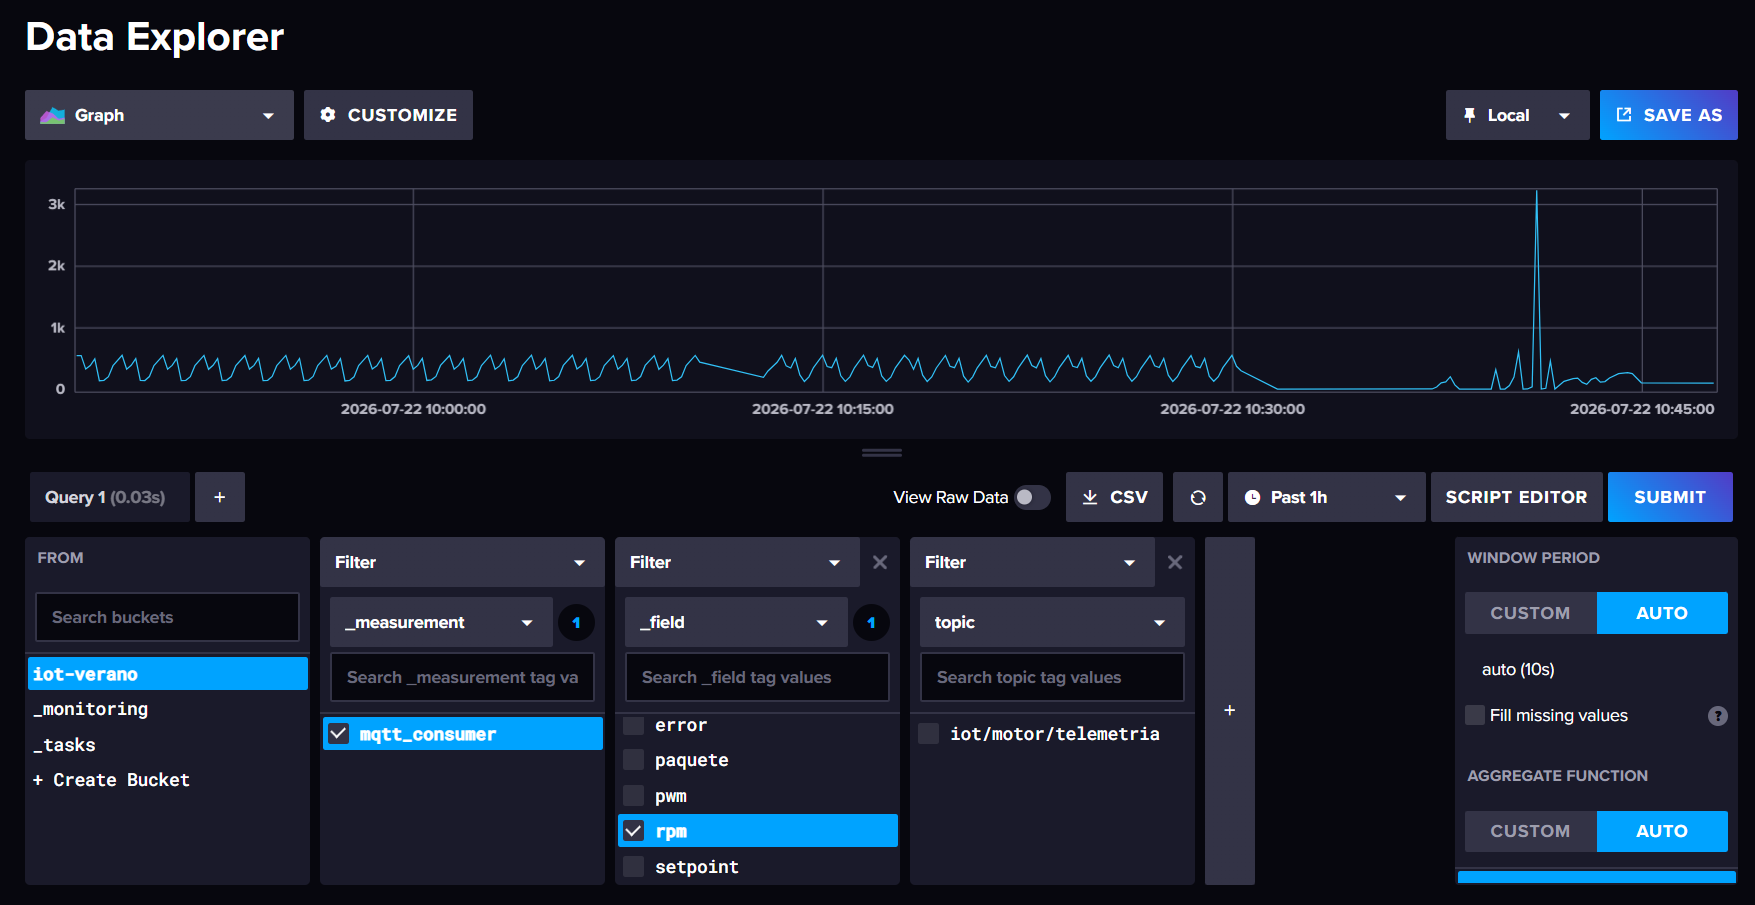
\includegraphics[width=0.85\textwidth]{CapturaInflux.png}
   \caption{InfluxDB Data Explorer mostrando los measurements del motor}
 \end{figure}

\textbf{Descripci\'on:}
Esta captura muestra el data explorer de Influx. Nos permite ver la informacion enviada desde nuestro motor.

\subsubsection{Dashboard completo de Grafana}

 \begin{figure}[H]
   \centering
   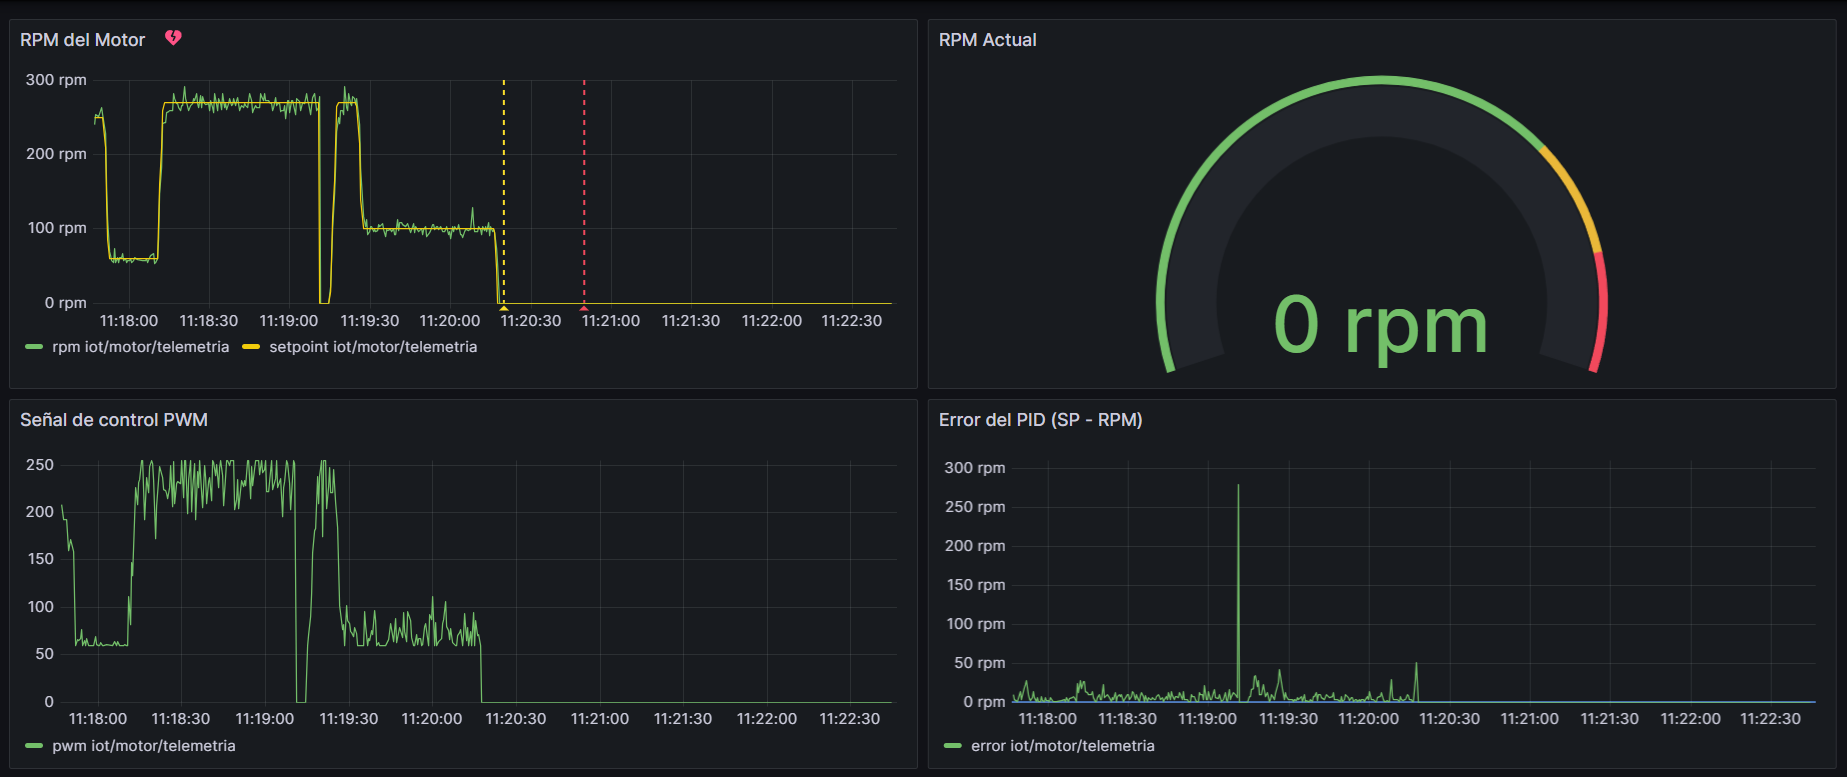
\includegraphics[width=0.85\textwidth]{CapturaGrafana.png}
   \caption{Dashboard de Grafana con los 4 paneles del motor en tiempo real}
 \end{figure}

\textbf{Descripci\'on:}
Esta captura nos muestra la dashboard de Grafana con la que podemos monitorear todos nuestros datos en tiempo real.

\subsection{Consultas Flux utilizadas}

\begin{instruccion}
  Pega las consultas Flux reales que usaste en cada panel de Grafana.
\end{instruccion}

\subsubsection{Panel RPM + Setpoint}

\begin{lstlisting}[style=flux, caption={Consulta Flux --- Panel RPM y Setpoint}]
from ( bucket : "iot-verano")
  |> range ( start : v.timeRangeStart , stop : v.timeRangeStop )
  |> filter ( fn : ( r ) => r ["_field"] == "rpm" or r ["_field"] == "setpoint")
  |> aggregateWindow ( every : v.windowPeriod , fn : mean , createEmpty : false )
  |> yield ( name : "motor")
\end{lstlisting}

\subsubsection{Panel Error del PID}

\begin{lstlisting}[style=flux, caption={Consulta Flux --- Panel Error}]
from ( bucket : "iot-verano")
  |> range ( start : v.timeRangeStart , stop : v.timeRangeStop )
  |> filter ( fn : ( r ) => r ["_field"] == "error")
  |> aggregateWindow ( every : v.windowPeriod , fn : mean , createEmpty : false )
  |> yield ( name : "error_pid")
\end{lstlisting}

\subsubsection{Panel Señal PWM}

\begin{lstlisting}[style=flux, caption={Consulta Flux --- Panel PWM}]
from ( bucket : "iot-verano")
  |> range ( start : v.timeRangeStart , stop : v.timeRangeStop )
  |> filter ( fn : ( r ) => r ["_field"] == "pwm")
  |> aggregateWindow ( every : v.windowPeriod , fn : mean , createEmpty : false )
  |> yield ( name : "pwm_control")
\end{lstlisting}

\subsection{Experimento de escalón --- datos de Grafana}

\begin{instruccion}
  Completa la tabla con los valores reales que observaste en Grafana
  durante el experimento de escal\'on. Esperar al menos 20 segundos
  en cada setpoint antes de anotar.
\end{instruccion}

\begin{table}[H]
  \centering
  \begin{tabular}{>{\centering}p{2cm}
                  >{\centering}p{2.5cm}
                  >{\centering}p{2.5cm}
                  >{\centering}p{2cm}
                  p{3.8cm}}
    \toprule
    \textbf{Setpoint} &
    \textbf{RPM estado} &
    \textbf{Error} &
    \textbf{PWM} &
    \textbf{Observaci\'on del equipo} \\
    \textbf{(RPM)} &
    \textbf{estacionario} &
    \textbf{residual (RPM)} &
    \textbf{estacionario} & \\
    \midrule
    60& 66.64& 6.64&
          63& \cellcolor{grayLight} \\[1.2em]
    100& 106.81& 6.81&
          104& \cellcolor{grayLight} \\[1.2em]
    150& 157.72& 7.52&
          158& \cellcolor{grayLight} \\[1.2em]
    200& 209.06& 9.06&
          215& \cellcolor{grayLight} \\[1.2em]
    \bottomrule
  \end{tabular}
  \caption{Respuesta del PID a distintos setpoints --- datos de Grafana}
\end{table}

\subsection{Registro del Serial Monitor}

\begin{instruccion}
  Copia un fragmento representativo del Serial Monitor que incluya:
  arranque del sistema, conexi\'on WiFi y MQTT, al menos 5 ciclos
  de publicaci\'on y la recepci\'on de un nuevo setpoint.
\end{instruccion}

\begin{lstlisting}[language={}, caption={Fragmento del Serial Monitor}]
>> [WIFI] Conectando a 'Jaime\_S24\_FE'.... 
>> [WIFI] OK - IP: 10.198.97.138 
>> [MQTT] Conectando al broker... OK 
--- ¡Sistema PID IoT con Modo Test Listo! --- 
--- COMANDOS DE CONTROL DISPONIBLES ---  
S<valor> : Definir RPM objetivo (Ej: S120)  
KP<valor> : Modificar Kp (Ej: KP2.5)  
KI<valor> : Modificar Ki (Ej: KI1.8)  
KD<valor> : Modificar Kd (Ej: KD0.05)  
C : Ver constantes PID actuales  
T : EJECUTAR MODO TEST (5s con impresiones normalizadas)  
R : ENCENDER / REANUDAR (Modo continuo)  
A : APAGADO GRADUAL (Bajada suave y progresiva)  
E : PARO DE EMERGENCIA (Freno total instantáneo)  
D : Cambiar sentido de giro 
--------------------------------------- 
Target:0.00,Actual:3.21,PWM:0\_APAGADO 
Target:0.00,Actual:128.34,PWM:0\_APAGADO 
Target:0.00,Actual:41.71,PWM:0\_APAGADO 
Target:0.00,Actual:195.72,PWM:0\_APAGADO 
Target:0.00,Actual:173.26,PWM:0\_APAGADO 
\end{lstlisting}

\newpage

% =============================================================================
\section{Análisis y discusión}
% =============================================================================

\begin{instruccion}
  No repitas los resultados --- interpr\'etalos. Explica el
  \textbf{por qu\'e} de lo que observaste. M\'inimo 2 oraciones
  por pregunta.
\end{instruccion}

% ── A1 ────────────────────────────────────────────────────────────────────────
\subsection{Análisis del error residual en estado estacionario}

\textit{Observando la tabla del experimento de escal\'on:
¿el motor llega exactamente al setpoint (error = 0)?
¿Cu\'al de los t\'erminos del PID es el responsable de eliminar
el error residual y por qu\'e?}

EL Error residual es eliminado por la parte integrativa ya que esta es la encargada de "jalar el sistema hasta su objetivo"

% ── A2 ────────────────────────────────────────────────────────────────────────
\subsection{Análisis del sobreimpulso}

\textit{¿Observaron sobreimpulso al cambiar el setpoint de 200 a 600 RPM?
¿C\'omo se ve en la gr\'afica de Grafana? ¿Qu\'e par\'ametro del PID
reducir\'ias para disminuirlo y qu\'e consecuencia tendr\'ia en la
velocidad de respuesta?}

Si, en la grafica se ve como un pico que sobrepasa el valor objetivo. Se puede redicir al disminuir el valor de la Kp, ya que esta es la que le da este impulso al sistema. Esto va a provocar que el sistema sea mas lento en responder.

% ── A3 ────────────────────────────────────────────────────────────────────────
\subsection{Análisis de la señal PWM}

\textit{¿El PWM es constante en estado estacionario o sigue variando?
Explica por qu\'e con base en los t\'erminos del PID.
¿Cu\'al de los 3 t\'erminos es el dominante en estado estacionario?}

El PWM siempre esta variando ya que el motor no es exacto, y va generando un error. Al generar este error, la parte integrativa va aumentando y, por esta razon, el PWM siempre cambia para poder compensar este error.
La parte Integrativa es la mas dominante durante el estado estacionario.

% ── A4 ────────────────────────────────────────────────────────────────────────
\subsection{Latencia del pipeline}

\textit{Cuando enviaron un nuevo setpoint por MQTT desde la terminal,
¿cu\'anto tiempo tard\'o en reflejarse el cambio en Grafana?
Descompon el tiempo estimado en cada etapa del pipeline:
terminal $\to$ MQTT $\to$ ESP32 $\to$ PID $\to$ motor $\to$
MQTT $\to$ InfluxDB $\to$ Grafana.}

\begin{table}[H]
  \centering
  \begin{tabular}{p{6cm} >{\centering\arraybackslash}p{3cm} p{4.5cm}}
    \toprule
    \textbf{Etapa} & \textbf{Latencia estimada} & \textbf{Justificaci\'on} \\
    \midrule
    Terminal $\to$ Broker MQTT   & ~10 - 20 ms& Latencia típica de transmisión en una red local WiFi.\\[1em]
    Broker $\to$ ESP32           & ~10 - 20 ms& Latencia de red WiFi local desde el broker al suscriptor (ESP32).\\[1em]
    ESP32 procesa el setpoint    & \cellcolor{grayLight}$\leq$ 10 ms & Loop del PID \\[1em]
    Motor responde (hasta 63\%)  & ~150 - 300 ms& $\approx \tau$ del motor \\[1em]
    ESP32 $\to$ InfluxDB (v\'ia MQTT + Telegraf) & ~500 - 550 ms& Se publican datos cada 500ms, y telegraf puede tener latencia de 50ms\\[1em]
    InfluxDB $\to$ Grafana (refresco) & 5000 ms& Intervalo configurado \\[1em]
    \midrule
    \textbf{Total percibido en Grafana} & ~5.7 - 6.0 s& \\[1em]
    \bottomrule
  \end{tabular}
  \caption{Desglose de latencia del pipeline completo}
\end{table}

% ── A5 ────────────────────────────────────────────────────────────────────────
\subsection{¿El PID está bien sintonizado? Tu criterio}

\textit{Propón un criterio num\'erico propio para evaluar si tu PID
est\'a bien sintonizado, basado en los datos de Grafana.
¿Tu PID cumple ese criterio? Justifica con valores concretos
de la tabla de resultados.}

\textbf{Mi criterio de sintonización:}
En estado estacionario, el error debe de ser de +- 15 rpm, ademas de asegurar que el sobreimpulso sea menor a 5\% del valor deseado.

\textbf{Evaluación del PID contra el criterio:}
Nuestro controlador PID es casi bueno. El error que tenemos si fluctua dentro de +-15 rmp, pero llega a tener picos de hasta 20 rpm, por lo que no es del todo ideal. 
En cuanto al sobreimpulso, logramos que el motor siguiera a perfectamente el objetivo durante un cambio.

\newpage

% =============================================================================
\section{Preguntas de análisis técnico}
% =============================================================================

\begin{instruccion}
  Responde con fundamento t\'ecnico. Conecta cada respuesta
  con lo que observaste en la pr\'actica.
\end{instruccion}

\begin{enumerate}[leftmargin=1.5cm, label=\textbf{P\arabic*.}, itemsep=0.4cm]

  % P1
  \item \textbf{En el c\'odigo del PID, si eliminas el \texttt{integral = 0}
        del callback de setpoint y cambias de 200 a 600 RPM,
        ¿qu\'e esperar\'ias ver en la gr\'afica de Grafana durante
        los primeros segundos? Explica el fen\'omeno.}

    Se observar\'ia un sobreimpulso (\textit{overshoot}) masivo en la gr\'afica. Al cambiar bruscamente a 600 RPM, se genera un error positivo muy grande. Mientras el motor vence su inercia para acelerar, este gran error se ir\'a acumulando r\'apidamente en la variable \texttt{integral} (fen\'omeno conocido como \textit{Integral Windup}). Cuando el motor finalmente alcance las 600 RPM, el t\'ermino integral ser\'a tan alto que forzar\'a al PWM a seguir al m\'aximo, causando que el motor se pase de largo (ej. llegando a 700 RPM) antes de que el error negativo logre ``desenrollar'' esa acumulaci\'on y estabilizar el sistema.
  

  % P2
  \item \textbf{¿Por qu\'e el loop del PID corre cada 10 ms pero
        MQTT publica cada 500 ms? Si publicaras cada 10 ms
        (igual que el PID), ¿qu\'e problemas podr\'ian aparecer
        en el pipeline?}

El PID necesita correr a alta frecuencia (100 Hz / 10 ms) para poder reaccionar en tiempo real a las perturbaciones mec\'anicas y mantener la estabilidad del sistema f\'isico. Por otro lado, la telemetr\'ia es s\'olo para supervisi\'on humana. Si MQTT publicara cada 10 ms, enviar\'iamos 100 mensajes por segundo. Esto provocar\'ia varios problemas: saturaci\'on del buffer de red del ESP32 (causando cuelgues o reinicios por \textit{Watchdog}), congesti\'on excesiva en el broker MQTT, sobrecarga de escritura en la base de datos InfluxDB, e interrupciones en el propio ciclo del PID, arruinando el control del motor.


  % P3
  \item \textbf{Escribe la consulta Flux que retorna el valor
        m\'aximo de error que tuvo el motor en la \'ultima hora.
        Explica c\'omo la usar\'ias para evaluar la calidad de tu
        sintonizaci\'on.}

  \begin{lstlisting}[style=flux, numbers=none]
from(bucket: "nombre_de_tu_bucket")
  |> range(start: -1h)
  |> filter(fn: (r) => r["_measurement"] == "mqtt_consumer")
  |> filter(fn: (r) => r["_field"] == "error")
  |> max()
  \end{lstlisting}

    Esta consulta filtra los datos de la \'ultima hora para el campo \texttt{error} y extrae exclusivamente el pico m\'as alto registrado. En t\'erminos de sintonizaci\'on, este valor representa el peor escenario de desviaci\'on (ya sea por un cambio de \textit{setpoint} o una perturbaci\'on f\'isica). Si el valor devuelto por \texttt{max()} es excesivamente alto, indica que el PID es muy lento para reaccionar o sufre de un sobreimpulso severo, sugiriendo que se debe ajustar la ganancia Proporcional ($K_p$) o Integral ($K_i$).
  

  % P4
  \item \textbf{¿Qu\'e pasar\'ia con el control del motor si el
        WiFi se cae mientras el motor est\'a girando a 500 RPM?
        ¿C\'omo est\'a protegido el sistema ante esa situaci\'on
        en el c\'odigo que escribieron?}

    El motor seguir\'a girando de forma estable a 500 RPM. El sistema est\'a protegido porque el lazo de control PID es un proceso local que se ejecuta de manera no bloqueante. En el c\'odigo, la lectura del encoder, los c\'alculos matem\'aticos y la escritura del PWM no dependen de funciones de red. S\'olo la publicaci\'on (\texttt{publicarTelemetria}) y la recepci\'on de comandos est\'an vinculadas al WiFi. Adem\'as, la l\'ogica de reconexi\'on est\'a diseñada para intentar recuperar la conexi\'on sin usar \texttt{delay()} que bloquee el ciclo principal, garantizando el control ininterrumpido.
  

  % P5
  \item \textbf{El campo \texttt{nodo} en el JSON se convierte en
        Tag en InfluxDB. Si el sistema tuviera 10 motores
        con 10 ESP32 publicando al mismo topic, ¿c\'omo modificar\'ias
        la consulta Flux para ver solo el motor de tu equipo?}

  \begin{lstlisting}[style=flux, numbers=none]
from(bucket: "nombre_de_tu_bucket")
  |> range(start: v.timeRangeStart, stop: v.timeRangeStop)
  |> filter(fn: (r) => r["_measurement"] == "mqtt_consumer")
  |> filter(fn: (r) => r["_field"] == "rpm")
  |> filter(fn: (r) => r["nodo"] == "ESP32-Motor-PID")
  \end{lstlisting}

    A\~nadiendo un filtro espec\'ifico para la etiqueta (\textit{tag}) \texttt{nodo}. Al incluir \texttt{|> filter(fn: (r) => r["nodo"] == "ESP32-Motor-PID")}, le indicamos a InfluxDB que discrimine y descarte los paquetes de los dem\'as equipos, graficando \'unicamente la serie de tiempo que coincide exactamente con el identificador de nuestro ESP32, evitando que las gr\'aficas se empalmen.
  

  % P6
  \item \textbf{¿Qu\'e diferencia hay entre la frecuencia de control
        del PID (100 Hz en el ESP32) y la frecuencia de muestreo
        en Grafana? ¿Cu\'al es el l\'imite te\'orico de la frecuencia
        de muestreo en Grafana con la configuraci\'on actual
        (refresco cada 5 s, intervalo MQTT 500 ms)?}

    La frecuencia de control (100 Hz) determina qu\'e tan r\'apido el hardware ajusta la potencia f\'isica del motor bas\'andose en sensores locales; es un proceso de tiempo real. La frecuencia de muestreo en Grafana es simplemente la tasa a la que podemos observar esos datos visualmente. Con la configuraci\'on actual, Grafana actualiza el panel cada 5 segundos, pero el l\'imite te\'orico de resoluci\'on de los datos almacenados es de 2 Hz (un punto cada 500 ms), ya que esa es la tasa a la que el ESP32 publica en MQTT. Grafana no puede mostrar eventos que duren menos de 500 ms, aunque el PID los haya corregido localmente en milisegundos.
  

\end{enumerate}

\end{enumerate}

% =============================================================================
\section{Conclusiones}
% =============================================================================

\begin{instruccion}
  Escribe m\'inimo \textbf{3 conclusiones numeradas}.
  Cada una debe: ser verificable con datos reales de la pr\'actica,
  conectar con alguno de los conceptos del marco te\'orico, y no
  ser una opini\'on general.
\end{instruccion}

\begin{enumerate}[leftmargin=1.5cm, itemsep=0.5cm]
  \item La comunicaci\'on a trav\'es del broker MQTT hasta InfluxDB fu\'e exitosa.  Por lo tanto la visualizaci\'on del contenido de RPM, objetivo de esta pr\'actica estuvo bien logrado. Y aunque se presentaron diversas dificultades como el hecho de que se tuvo apagar el firewall de la computadora para lograr el correcto funcionamiento los resultados fueron los esperados, con un flujo de RPM a trav\'es del tiempo.
  \item Para el control PID se intent\'o realizar a trav\'es de una funci\'on de transferencia que se obtuvo de los datos descriptivos de un comportamiento controlado. Lamentablemente al no funcionar del todo y tener errores masivos conforme se aumentaban las revoluciones, optamos por hacer modifcaciones a trav\'es de prueba y error tomando los valores inicialmente obtenidos por la funci\'on de transferencia. Lo que al final fué lo que nos funcionó reduciendo el erorr ligeramente.
  \item El envio desde el ESP32 hasta Grafana sucedio con exito. Logramos leer los RPMs del motor y enviarlos a una interfaz grafica en tiempo real, ademas de configurar todo lo que necesitamos leer, como el setpoint y las PWMs con las que controlamos el motor. Costo mucho trabajo ya que tuvimos muchos problemas a lo largo del camino, como el WiFi no funcionando adecuadamente, o el firewall bloqueando las funciones.
\end{enumerate}

% =============================================================================
\section{Repositorio y entregables}
% =============================================================================

\begin{tabular}{rl}
  \textbf{URL del repositorio:} & https://github.com/0263136-JVR/Practicas-IoT\\[0.6em]
  \textbf{Carpeta del c\'odigo:} & Practica 3/Codigo PID-MQTT\\[0.6em]
  \textbf{Fecha del \'ultimo commit:} & 23/07/26\\
\end{tabular}

\vspace{0.5cm}

\begin{mdframed}[backgroundcolor=amberLight,linecolor=amberMain,linewidth=1pt,
  innerleftmargin=12pt,innerrightmargin=12pt,
  innertopmargin=8pt,innerbottommargin=8pt]
  \textbf{\color{amberMain}Lista de verificaci\'on antes de entregar:}
  \begin{multicols}{2}
  \begin{itemize}[leftmargin=1.5cm, label=$\square$, itemsep=2pt]
    \item PDF compilado sin errores
    \item Tabla de conexiones completa
    \item C\'odigo real pegado (secci\'on 4)
    \item Tabla de par\'ametros PID completa
    \item 3 capturas de pantalla insertadas
    \item Consultas Flux pegadas
    \item Tabla del experimento de escal\'on con datos reales
    \item Serial Monitor pegado
    \item 6 preguntas de an\'alisis respondidas
    \item Tabla de latencia del pipeline completa
    \item M\'inimo 3 conclusiones
    \item C\'odigo y \texttt{.tex} en GitHub
  \end{itemize}
  \end{multicols}
\end{mdframed}

\vspace{0.4cm}

% =============================================================================
\section*{Referencias}
% =============================================================================

\begin{instruccion}
  M\'inimo 3 fuentes. Incluir el datasheet del TB6612FNG,
  la documentaci\'on de InfluxDB y al menos una fuente adicional.
\end{instruccion}

\begin{thebibliography}{9}
  \bibitem{drv8833}  Toshiba. \textit{DRV8833 Datasheet}. 2011. https://www.alldatasheet.com/html-pdf/437529/TI1/DRV8833/54/1/DRV8833.html
  \bibitem{influx}  InfluxData. \textit{InfluxDB v2 Documentation}. 2024.
                   https://docs.influxdata.com
  \bibitem{windup} Windup. Controlguru. (s. f.). Integral (Reset) Windup, Jacketing Logic and the Velocity PI Form – Control Guru. https://controlguru.com/integral-reset-windup-jacketing-logic-and-the-velocity-pi-form/
\end{thebibliography}

\end{document}
